% Created by tikzDevice version 0.12.3.1 on 2022-05-11 22:45:10
% !TEX encoding = UTF-8 Unicode
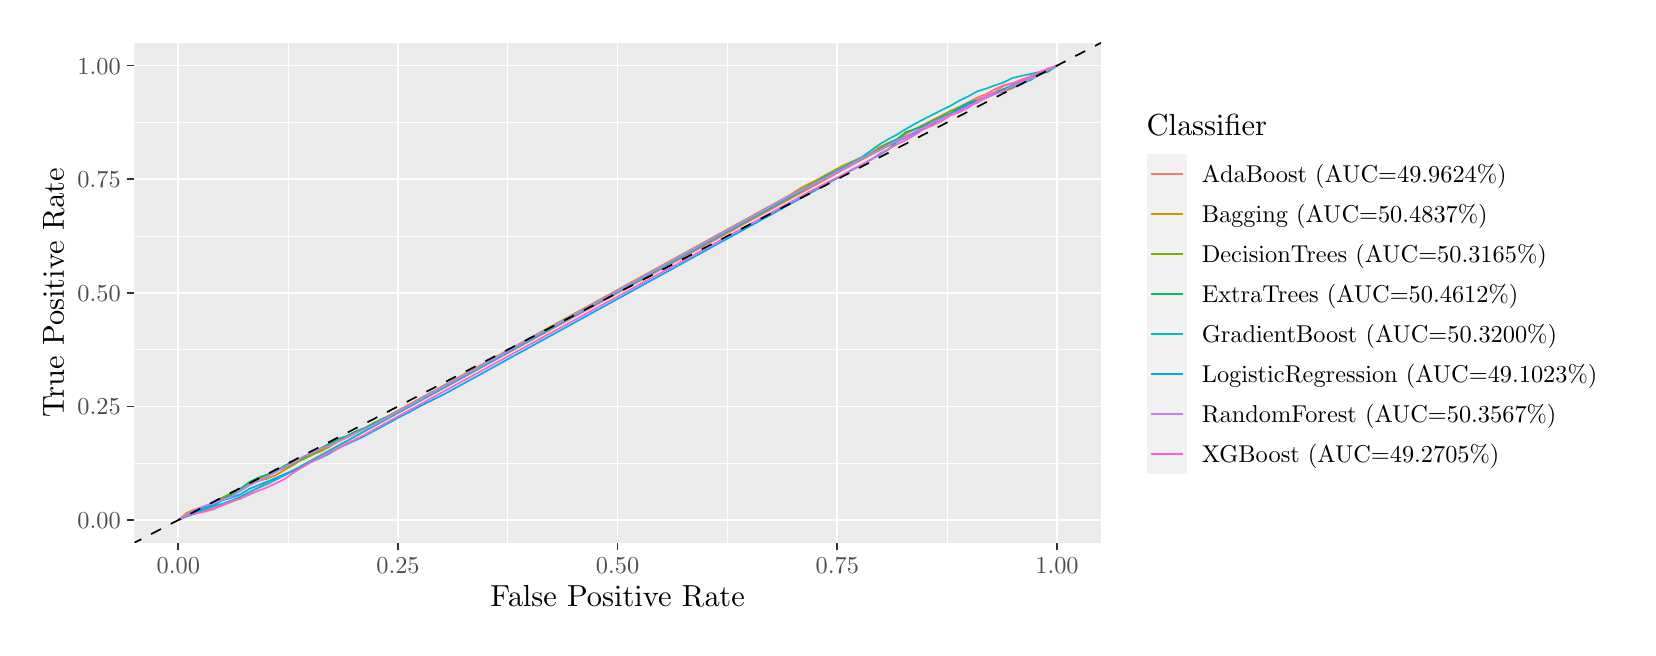
\begin{tikzpicture}[x=1pt,y=1pt]
\definecolor{fillColor}{RGB}{255,255,255}
\path[use as bounding box,fill=fillColor,fill opacity=0.00] (0,0) rectangle (578.16,216.81);
\begin{scope}
\path[clip] (  0.00,  0.00) rectangle (578.16,216.81);
\definecolor{drawColor}{RGB}{255,255,255}
\definecolor{fillColor}{RGB}{255,255,255}

\path[draw=drawColor,line width= 0.6pt,line join=round,line cap=round,fill=fillColor] (  0.00,  0.00) rectangle (578.16,216.81);
\end{scope}
\begin{scope}
\path[clip] ( 38.56, 30.69) rectangle (387.81,211.31);
\definecolor{fillColor}{gray}{0.92}

\path[fill=fillColor] ( 38.56, 30.69) rectangle (387.81,211.31);
\definecolor{drawColor}{RGB}{255,255,255}

\path[draw=drawColor,line width= 0.3pt,line join=round] ( 38.56, 59.42) --
	(387.81, 59.42);

\path[draw=drawColor,line width= 0.3pt,line join=round] ( 38.56,100.47) --
	(387.81,100.47);

\path[draw=drawColor,line width= 0.3pt,line join=round] ( 38.56,141.52) --
	(387.81,141.52);

\path[draw=drawColor,line width= 0.3pt,line join=round] ( 38.56,182.57) --
	(387.81,182.57);

\path[draw=drawColor,line width= 0.3pt,line join=round] ( 94.12, 30.69) --
	( 94.12,211.31);

\path[draw=drawColor,line width= 0.3pt,line join=round] (173.50, 30.69) --
	(173.50,211.31);

\path[draw=drawColor,line width= 0.3pt,line join=round] (252.87, 30.69) --
	(252.87,211.31);

\path[draw=drawColor,line width= 0.3pt,line join=round] (332.25, 30.69) --
	(332.25,211.31);

\path[draw=drawColor,line width= 0.6pt,line join=round] ( 38.56, 38.90) --
	(387.81, 38.90);

\path[draw=drawColor,line width= 0.6pt,line join=round] ( 38.56, 79.95) --
	(387.81, 79.95);

\path[draw=drawColor,line width= 0.6pt,line join=round] ( 38.56,121.00) --
	(387.81,121.00);

\path[draw=drawColor,line width= 0.6pt,line join=round] ( 38.56,162.05) --
	(387.81,162.05);

\path[draw=drawColor,line width= 0.6pt,line join=round] ( 38.56,203.10) --
	(387.81,203.10);

\path[draw=drawColor,line width= 0.6pt,line join=round] ( 54.43, 30.69) --
	( 54.43,211.31);

\path[draw=drawColor,line width= 0.6pt,line join=round] (133.81, 30.69) --
	(133.81,211.31);

\path[draw=drawColor,line width= 0.6pt,line join=round] (213.18, 30.69) --
	(213.18,211.31);

\path[draw=drawColor,line width= 0.6pt,line join=round] (292.56, 30.69) --
	(292.56,211.31);

\path[draw=drawColor,line width= 0.6pt,line join=round] (371.94, 30.69) --
	(371.94,211.31);
\definecolor{drawColor}{RGB}{248,118,109}

\path[draw=drawColor,line width= 0.6pt,line join=round] ( 54.43, 38.90) --
	( 57.64, 40.61) --
	( 60.84, 41.70) --
	( 64.05, 42.51) --
	( 67.26, 43.21) --
	( 70.47, 44.29) --
	( 73.67, 45.43) --
	( 76.88, 47.23) --
	( 80.09, 48.80) --
	( 83.29, 50.62) --
	( 86.50, 52.58) --
	( 89.71, 54.15) --
	( 92.92, 55.50) --
	( 96.12, 56.97) --
	( 99.33, 58.72) --
	(102.54, 60.47) --
	(105.74, 62.23) --
	(108.95, 63.98) --
	(112.16, 65.73) --
	(115.37, 67.48) --
	(118.57, 69.23) --
	(121.78, 70.98) --
	(124.99, 72.74) --
	(128.19, 74.49) --
	(131.40, 76.24) --
	(134.61, 77.99) --
	(137.82, 79.74) --
	(141.02, 81.50) --
	(144.23, 83.25) --
	(147.44, 85.00) --
	(150.64, 86.75) --
	(153.85, 88.50) --
	(157.06, 90.25) --
	(160.27, 92.01) --
	(163.47, 93.76) --
	(166.68, 95.51) --
	(169.89, 97.26) --
	(173.09, 99.01) --
	(176.30,100.77) --
	(179.51,102.52) --
	(182.72,104.27) --
	(185.92,106.02) --
	(189.13,107.77) --
	(192.34,109.52) --
	(195.54,111.28) --
	(198.75,113.03) --
	(201.96,114.78) --
	(205.17,116.53) --
	(208.37,118.28) --
	(211.58,120.04) --
	(214.79,121.79) --
	(217.99,123.54) --
	(221.20,125.29) --
	(224.41,127.04) --
	(227.62,128.79) --
	(230.82,130.55) --
	(234.03,132.30) --
	(237.24,134.05) --
	(240.44,135.80) --
	(243.65,137.55) --
	(246.86,139.31) --
	(250.07,141.06) --
	(253.27,142.81) --
	(256.48,144.56) --
	(259.69,146.31) --
	(262.90,148.06) --
	(266.10,149.82) --
	(269.31,151.57) --
	(272.52,153.32) --
	(275.72,155.07) --
	(278.93,156.82) --
	(282.14,158.58) --
	(285.35,160.33) --
	(288.55,162.08) --
	(291.76,163.83) --
	(294.97,165.58) --
	(298.17,167.33) --
	(301.38,169.09) --
	(304.59,170.84) --
	(307.80,172.59) --
	(311.00,174.34) --
	(314.21,176.35) --
	(317.42,178.45) --
	(320.62,180.21) --
	(323.83,181.79) --
	(327.04,183.48) --
	(330.25,185.07) --
	(333.45,186.69) --
	(336.66,188.18) --
	(339.87,189.82) --
	(343.07,191.54) --
	(346.28,192.76) --
	(349.49,194.57) --
	(352.70,195.99) --
	(355.90,196.68) --
	(359.11,198.08) --
	(362.32,199.10) --
	(365.52,200.17) --
	(368.73,201.53) --
	(371.94,203.10);
\definecolor{drawColor}{RGB}{205,150,0}

\path[draw=drawColor,line width= 0.6pt,line join=round] ( 54.43, 38.90) --
	( 57.64, 41.59) --
	( 60.84, 42.87) --
	( 64.05, 43.92) --
	( 67.26, 44.82) --
	( 70.47, 46.48) --
	( 73.67, 47.55) --
	( 76.88, 49.40) --
	( 80.09, 51.42) --
	( 83.29, 52.98) --
	( 86.50, 53.83) --
	( 89.71, 55.14) --
	( 92.92, 57.03) --
	( 96.12, 58.83) --
	( 99.33, 61.03) --
	(102.54, 62.44) --
	(105.74, 63.55) --
	(108.95, 65.30) --
	(112.16, 67.21) --
	(115.37, 68.72) --
	(118.57, 70.31) --
	(121.78, 71.93) --
	(124.99, 73.59) --
	(128.19, 75.35) --
	(131.40, 77.12) --
	(134.61, 78.88) --
	(137.82, 80.64) --
	(141.02, 82.41) --
	(144.23, 84.17) --
	(147.44, 85.94) --
	(150.64, 87.70) --
	(153.85, 89.46) --
	(157.06, 91.23) --
	(160.27, 92.99) --
	(163.47, 94.75) --
	(166.68, 96.52) --
	(169.89, 98.28) --
	(173.09,100.05) --
	(176.30,101.81) --
	(179.51,103.57) --
	(182.72,105.34) --
	(185.92,107.10) --
	(189.13,108.86) --
	(192.34,110.63) --
	(195.54,112.39) --
	(198.75,114.16) --
	(201.96,115.92) --
	(205.17,117.68) --
	(208.37,119.45) --
	(211.58,121.21) --
	(214.79,122.97) --
	(217.99,124.74) --
	(221.20,126.50) --
	(224.41,128.27) --
	(227.62,130.03) --
	(230.82,131.79) --
	(234.03,133.56) --
	(237.24,135.32) --
	(240.44,137.08) --
	(243.65,138.85) --
	(246.86,140.61) --
	(250.07,142.38) --
	(253.27,144.14) --
	(256.48,145.90) --
	(259.69,147.67) --
	(262.90,149.43) --
	(266.10,151.19) --
	(269.31,152.96) --
	(272.52,154.73) --
	(275.72,156.52) --
	(278.93,158.62) --
	(282.14,160.32) --
	(285.35,161.91) --
	(288.55,163.71) --
	(291.76,165.46) --
	(294.97,167.16) --
	(298.17,168.57) --
	(301.38,169.97) --
	(304.59,171.30) --
	(307.80,173.65) --
	(311.00,175.19) --
	(314.21,176.17) --
	(317.42,177.64) --
	(320.62,178.95) --
	(323.83,180.84) --
	(327.04,182.10) --
	(330.25,184.10) --
	(333.45,185.46) --
	(336.66,186.92) --
	(339.87,188.73) --
	(343.07,190.16) --
	(346.28,191.36) --
	(349.49,192.90) --
	(352.70,193.81) --
	(355.90,194.88) --
	(359.11,196.92) --
	(362.32,199.29) --
	(365.52,200.32) --
	(368.73,201.85) --
	(371.94,203.10);
\definecolor{drawColor}{RGB}{124,174,0}

\path[draw=drawColor,line width= 0.6pt,line join=round] ( 54.43, 38.90) --
	( 57.64, 40.53) --
	( 60.84, 42.16) --
	( 64.05, 43.80) --
	( 67.26, 45.43) --
	( 70.47, 47.07) --
	( 73.67, 48.70) --
	( 76.88, 50.33) --
	( 80.09, 51.97) --
	( 83.29, 53.60) --
	( 86.50, 55.22) --
	( 89.71, 56.53) --
	( 92.92, 57.70) --
	( 96.12, 59.27) --
	( 99.33, 60.69) --
	(102.54, 62.26) --
	(105.74, 64.15) --
	(108.95, 66.01) --
	(112.16, 67.55) --
	(115.37, 68.87) --
	(118.57, 70.66) --
	(121.78, 72.02) --
	(124.99, 73.96) --
	(128.19, 75.42) --
	(131.40, 76.93) --
	(134.61, 78.40) --
	(137.82, 80.17) --
	(141.02, 81.92) --
	(144.23, 83.68) --
	(147.44, 85.43) --
	(150.64, 87.18) --
	(153.85, 88.94) --
	(157.06, 90.69) --
	(160.27, 92.44) --
	(163.47, 94.20) --
	(166.68, 95.95) --
	(169.89, 97.70) --
	(173.09, 99.46) --
	(176.30,101.21) --
	(179.51,102.96) --
	(182.72,104.72) --
	(185.92,106.47) --
	(189.13,108.22) --
	(192.34,109.98) --
	(195.54,111.73) --
	(198.75,113.48) --
	(201.96,115.24) --
	(205.17,116.99) --
	(208.37,118.74) --
	(211.58,120.50) --
	(214.79,122.25) --
	(217.99,124.00) --
	(221.20,125.76) --
	(224.41,127.51) --
	(227.62,129.26) --
	(230.82,131.02) --
	(234.03,132.77) --
	(237.24,134.52) --
	(240.44,136.28) --
	(243.65,138.03) --
	(246.86,139.78) --
	(250.07,141.54) --
	(253.27,143.29) --
	(256.48,145.04) --
	(259.69,146.80) --
	(262.90,148.55) --
	(266.10,150.30) --
	(269.31,152.06) --
	(272.52,153.81) --
	(275.72,155.56) --
	(278.93,157.32) --
	(282.14,159.07) --
	(285.35,160.82) --
	(288.55,162.58) --
	(291.76,164.34) --
	(294.97,166.04) --
	(298.17,167.73) --
	(301.38,169.34) --
	(304.59,170.91) --
	(307.80,172.47) --
	(311.00,174.11) --
	(314.21,175.85) --
	(317.42,177.24) --
	(320.62,178.83) --
	(323.83,181.58) --
	(327.04,183.28) --
	(330.25,184.78) --
	(333.45,186.68) --
	(336.66,188.06) --
	(339.87,189.41) --
	(343.07,190.62) --
	(346.28,192.01) --
	(349.49,193.31) --
	(352.70,194.66) --
	(355.90,195.63) --
	(359.11,197.28) --
	(362.32,198.36) --
	(365.52,200.08) --
	(368.73,201.45) --
	(371.94,203.10);
\definecolor{drawColor}{RGB}{0,190,103}

\path[draw=drawColor,line width= 0.6pt,line join=round] ( 54.43, 38.90) --
	( 57.64, 40.52) --
	( 60.84, 42.15) --
	( 64.05, 43.75) --
	( 67.26, 45.12) --
	( 70.47, 46.37) --
	( 73.67, 48.24) --
	( 76.88, 50.15) --
	( 80.09, 52.62) --
	( 83.29, 54.20) --
	( 86.50, 55.31) --
	( 89.71, 56.48) --
	( 92.92, 58.59) --
	( 96.12, 60.13) --
	( 99.33, 61.36) --
	(102.54, 63.16) --
	(105.74, 64.76) --
	(108.95, 66.45) --
	(112.16, 68.25) --
	(115.37, 69.25) --
	(118.57, 71.01) --
	(121.78, 72.16) --
	(124.99, 73.68) --
	(128.19, 75.38) --
	(131.40, 76.78) --
	(134.61, 78.34) --
	(137.82, 80.22) --
	(141.02, 82.00) --
	(144.23, 83.76) --
	(147.44, 85.52) --
	(150.64, 87.29) --
	(153.85, 89.05) --
	(157.06, 90.82) --
	(160.27, 92.58) --
	(163.47, 94.35) --
	(166.68, 96.11) --
	(169.89, 97.88) --
	(173.09, 99.64) --
	(176.30,101.40) --
	(179.51,103.17) --
	(182.72,104.93) --
	(185.92,106.70) --
	(189.13,108.46) --
	(192.34,110.23) --
	(195.54,111.99) --
	(198.75,113.76) --
	(201.96,115.52) --
	(205.17,117.29) --
	(208.37,119.05) --
	(211.58,120.81) --
	(214.79,122.58) --
	(217.99,124.34) --
	(221.20,126.11) --
	(224.41,127.87) --
	(227.62,129.64) --
	(230.82,131.40) --
	(234.03,133.17) --
	(237.24,134.93) --
	(240.44,136.69) --
	(243.65,138.46) --
	(246.86,140.22) --
	(250.07,141.99) --
	(253.27,143.75) --
	(256.48,145.52) --
	(259.69,147.28) --
	(262.90,149.05) --
	(266.10,150.81) --
	(269.31,152.57) --
	(272.52,154.34) --
	(275.72,156.10) --
	(278.93,157.87) --
	(282.14,159.63) --
	(285.35,161.26) --
	(288.55,163.24) --
	(291.76,164.73) --
	(294.97,166.43) --
	(298.17,168.03) --
	(301.38,169.62) --
	(304.59,171.25) --
	(307.80,172.97) --
	(311.00,174.95) --
	(314.21,176.57) --
	(317.42,179.10) --
	(320.62,180.13) --
	(323.83,181.46) --
	(327.04,182.72) --
	(330.25,184.48) --
	(333.45,185.77) --
	(336.66,187.82) --
	(339.87,189.62) --
	(343.07,190.60) --
	(346.28,191.63) --
	(349.49,192.93) --
	(352.70,194.55) --
	(355.90,196.04) --
	(359.11,197.04) --
	(362.32,197.81) --
	(365.52,200.08) --
	(368.73,200.88) --
	(371.94,203.10);
\definecolor{drawColor}{RGB}{0,191,196}

\path[draw=drawColor,line width= 0.6pt,line join=round] ( 54.43, 38.90) --
	( 57.64, 40.24) --
	( 60.84, 41.27) --
	( 64.05, 42.78) --
	( 67.26, 43.94) --
	( 70.47, 44.78) --
	( 73.67, 45.97) --
	( 76.88, 47.34) --
	( 80.09, 48.98) --
	( 83.29, 50.47) --
	( 86.50, 51.83) --
	( 89.71, 53.48) --
	( 92.92, 55.11) --
	( 96.12, 56.89) --
	( 99.33, 58.66) --
	(102.54, 60.42) --
	(105.74, 62.19) --
	(108.95, 63.95) --
	(112.16, 65.72) --
	(115.37, 67.48) --
	(118.57, 69.25) --
	(121.78, 71.01) --
	(124.99, 72.78) --
	(128.19, 74.55) --
	(131.40, 76.31) --
	(134.61, 78.08) --
	(137.82, 79.84) --
	(141.02, 81.61) --
	(144.23, 83.37) --
	(147.44, 85.14) --
	(150.64, 86.90) --
	(153.85, 88.67) --
	(157.06, 90.44) --
	(160.27, 92.20) --
	(163.47, 93.97) --
	(166.68, 95.73) --
	(169.89, 97.50) --
	(173.09, 99.26) --
	(176.30,101.03) --
	(179.51,102.79) --
	(182.72,104.56) --
	(185.92,106.33) --
	(189.13,108.09) --
	(192.34,109.86) --
	(195.54,111.62) --
	(198.75,113.39) --
	(201.96,115.15) --
	(205.17,116.92) --
	(208.37,118.68) --
	(211.58,120.45) --
	(214.79,122.22) --
	(217.99,123.98) --
	(221.20,125.75) --
	(224.41,127.51) --
	(227.62,129.28) --
	(230.82,131.04) --
	(234.03,132.81) --
	(237.24,134.57) --
	(240.44,136.34) --
	(243.65,138.11) --
	(246.86,139.87) --
	(250.07,141.64) --
	(253.27,143.40) --
	(256.48,145.17) --
	(259.69,146.93) --
	(262.90,148.70) --
	(266.10,150.46) --
	(269.31,152.23) --
	(272.52,154.00) --
	(275.72,155.76) --
	(278.93,157.53) --
	(282.14,159.29) --
	(285.35,161.06) --
	(288.55,162.82) --
	(291.76,164.59) --
	(294.97,166.36) --
	(298.17,168.12) --
	(301.38,170.04) --
	(304.59,172.27) --
	(307.80,174.66) --
	(311.00,176.50) --
	(314.21,178.21) --
	(317.42,180.22) --
	(320.62,182.07) --
	(323.83,183.76) --
	(327.04,185.39) --
	(330.25,187.02) --
	(333.45,188.56) --
	(336.66,190.46) --
	(339.87,191.99) --
	(343.07,193.76) --
	(346.28,194.77) --
	(349.49,195.95) --
	(352.70,197.03) --
	(355.90,198.65) --
	(359.11,199.38) --
	(362.32,200.07) --
	(365.52,200.78) --
	(368.73,201.76) --
	(371.94,203.10);
\definecolor{drawColor}{RGB}{0,169,255}

\path[draw=drawColor,line width= 0.6pt,line join=round] ( 54.43, 38.90) --
	( 57.64, 40.63) --
	( 60.84, 41.70) --
	( 64.05, 43.42) --
	( 67.26, 44.21) --
	( 70.47, 46.05) --
	( 73.67, 46.96) --
	( 76.88, 48.17) --
	( 80.09, 50.12) --
	( 83.29, 51.48) --
	( 86.50, 52.79) --
	( 89.71, 54.00) --
	( 92.92, 55.47) --
	( 96.12, 56.65) --
	( 99.33, 58.17) --
	(102.54, 59.91) --
	(105.74, 61.25) --
	(108.95, 62.91) --
	(112.16, 64.82) --
	(115.37, 66.31) --
	(118.57, 67.75) --
	(121.78, 69.26) --
	(124.99, 71.01) --
	(128.19, 72.75) --
	(131.40, 74.45) --
	(134.61, 76.23) --
	(137.82, 77.83) --
	(141.02, 79.61) --
	(144.23, 81.27) --
	(147.44, 82.83) --
	(150.64, 84.43) --
	(153.85, 86.19) --
	(157.06, 87.95) --
	(160.27, 89.72) --
	(163.47, 91.48) --
	(166.68, 93.24) --
	(169.89, 95.00) --
	(173.09, 96.77) --
	(176.30, 98.53) --
	(179.51,100.29) --
	(182.72,102.05) --
	(185.92,103.82) --
	(189.13,105.58) --
	(192.34,107.34) --
	(195.54,109.10) --
	(198.75,110.87) --
	(201.96,112.63) --
	(205.17,114.39) --
	(208.37,116.15) --
	(211.58,117.92) --
	(214.79,119.68) --
	(217.99,121.44) --
	(221.20,123.20) --
	(224.41,124.97) --
	(227.62,126.73) --
	(230.82,128.49) --
	(234.03,130.25) --
	(237.24,132.02) --
	(240.44,133.78) --
	(243.65,135.54) --
	(246.86,137.30) --
	(250.07,139.07) --
	(253.27,140.83) --
	(256.48,142.59) --
	(259.69,144.35) --
	(262.90,146.12) --
	(266.10,147.88) --
	(269.31,149.64) --
	(272.52,151.40) --
	(275.72,153.17) --
	(278.93,154.93) --
	(282.14,156.69) --
	(285.35,158.45) --
	(288.55,160.22) --
	(291.76,161.98) --
	(294.97,163.74) --
	(298.17,165.51) --
	(301.38,167.27) --
	(304.59,169.11) --
	(307.80,170.83) --
	(311.00,172.77) --
	(314.21,175.73) --
	(317.42,177.11) --
	(320.62,178.84) --
	(323.83,180.41) --
	(327.04,182.24) --
	(330.25,183.88) --
	(333.45,185.51) --
	(336.66,187.29) --
	(339.87,189.08) --
	(343.07,190.15) --
	(346.28,191.74) --
	(349.49,193.06) --
	(352.70,194.16) --
	(355.90,195.40) --
	(359.11,196.55) --
	(362.32,198.10) --
	(365.52,199.78) --
	(368.73,201.39) --
	(371.94,203.10);
\definecolor{drawColor}{RGB}{199,124,255}

\path[draw=drawColor,line width= 0.6pt,line join=round] ( 54.43, 38.90) --
	( 57.64, 41.04) --
	( 60.84, 42.67) --
	( 64.05, 44.10) --
	( 67.26, 44.87) --
	( 70.47, 46.30) --
	( 73.67, 47.33) --
	( 76.88, 49.52) --
	( 80.09, 51.60) --
	( 83.29, 52.95) --
	( 86.50, 54.48) --
	( 89.71, 56.20) --
	( 92.92, 58.06) --
	( 96.12, 59.49) --
	( 99.33, 61.72) --
	(102.54, 63.09) --
	(105.74, 64.65) --
	(108.95, 65.77) --
	(112.16, 67.25) --
	(115.37, 68.84) --
	(118.57, 70.39) --
	(121.78, 71.78) --
	(124.99, 73.23) --
	(128.19, 75.02) --
	(131.40, 76.79) --
	(134.61, 78.55) --
	(137.82, 80.32) --
	(141.02, 82.08) --
	(144.23, 83.85) --
	(147.44, 85.61) --
	(150.64, 87.37) --
	(153.85, 89.14) --
	(157.06, 90.90) --
	(160.27, 92.67) --
	(163.47, 94.43) --
	(166.68, 96.20) --
	(169.89, 97.96) --
	(173.09, 99.73) --
	(176.30,101.49) --
	(179.51,103.25) --
	(182.72,105.02) --
	(185.92,106.78) --
	(189.13,108.55) --
	(192.34,110.31) --
	(195.54,112.08) --
	(198.75,113.84) --
	(201.96,115.61) --
	(205.17,117.37) --
	(208.37,119.13) --
	(211.58,120.90) --
	(214.79,122.66) --
	(217.99,124.43) --
	(221.20,126.19) --
	(224.41,127.96) --
	(227.62,129.72) --
	(230.82,131.49) --
	(234.03,133.25) --
	(237.24,135.01) --
	(240.44,136.78) --
	(243.65,138.54) --
	(246.86,140.31) --
	(250.07,142.07) --
	(253.27,143.84) --
	(256.48,145.60) --
	(259.69,147.36) --
	(262.90,149.13) --
	(266.10,150.89) --
	(269.31,152.71) --
	(272.52,154.59) --
	(275.72,156.24) --
	(278.93,157.85) --
	(282.14,159.31) --
	(285.35,161.02) --
	(288.55,162.62) --
	(291.76,164.31) --
	(294.97,165.84) --
	(298.17,167.62) --
	(301.38,169.61) --
	(304.59,171.18) --
	(307.80,172.60) --
	(311.00,174.39) --
	(314.21,176.06) --
	(317.42,177.30) --
	(320.62,179.25) --
	(323.83,180.68) --
	(327.04,182.54) --
	(330.25,184.02) --
	(333.45,185.30) --
	(336.66,186.70) --
	(339.87,188.49) --
	(343.07,189.61) --
	(346.28,191.49) --
	(349.49,192.77) --
	(352.70,193.94) --
	(355.90,195.80) --
	(359.11,196.86) --
	(362.32,198.43) --
	(365.52,199.57) --
	(368.73,201.61) --
	(371.94,203.10);
\definecolor{drawColor}{RGB}{255,97,204}

\path[draw=drawColor,line width= 0.6pt,line join=round] ( 54.43, 38.90) --
	( 57.64, 40.72) --
	( 60.84, 41.25) --
	( 64.05, 41.94) --
	( 67.26, 42.83) --
	( 70.47, 44.28) --
	( 73.67, 45.53) --
	( 76.88, 46.59) --
	( 80.09, 48.09) --
	( 83.29, 49.46) --
	( 86.50, 50.67) --
	( 89.71, 52.17) --
	( 92.92, 53.74) --
	( 96.12, 56.07) --
	( 99.33, 58.02) --
	(102.54, 59.90) --
	(105.74, 61.39) --
	(108.95, 63.38) --
	(112.16, 64.71) --
	(115.37, 66.61) --
	(118.57, 68.14) --
	(121.78, 69.70) --
	(124.99, 71.51) --
	(128.19, 73.26) --
	(131.40, 75.01) --
	(134.61, 76.77) --
	(137.82, 78.52) --
	(141.02, 80.27) --
	(144.23, 82.02) --
	(147.44, 83.77) --
	(150.64, 85.52) --
	(153.85, 87.27) --
	(157.06, 89.03) --
	(160.27, 90.78) --
	(163.47, 92.53) --
	(166.68, 94.28) --
	(169.89, 96.03) --
	(173.09, 97.78) --
	(176.30, 99.53) --
	(179.51,101.29) --
	(182.72,103.04) --
	(185.92,104.79) --
	(189.13,106.54) --
	(192.34,108.29) --
	(195.54,110.04) --
	(198.75,111.79) --
	(201.96,113.55) --
	(205.17,115.30) --
	(208.37,117.05) --
	(211.58,118.80) --
	(214.79,120.55) --
	(217.99,122.30) --
	(221.20,124.05) --
	(224.41,125.81) --
	(227.62,127.56) --
	(230.82,129.31) --
	(234.03,131.06) --
	(237.24,132.81) --
	(240.44,134.56) --
	(243.65,136.32) --
	(246.86,138.07) --
	(250.07,139.82) --
	(253.27,141.57) --
	(256.48,143.32) --
	(259.69,145.07) --
	(262.90,146.82) --
	(266.10,148.58) --
	(269.31,150.33) --
	(272.52,152.08) --
	(275.72,153.83) --
	(278.93,155.58) --
	(282.14,157.33) --
	(285.35,158.95) --
	(288.55,160.67) --
	(291.76,162.27) --
	(294.97,163.85) --
	(298.17,165.74) --
	(301.38,167.31) --
	(304.59,168.97) --
	(307.80,171.28) --
	(311.00,172.89) --
	(314.21,174.74) --
	(317.42,176.22) --
	(320.62,178.08) --
	(323.83,180.12) --
	(327.04,181.49) --
	(330.25,183.01) --
	(333.45,185.11) --
	(336.66,186.27) --
	(339.87,187.89) --
	(343.07,190.22) --
	(346.28,192.07) --
	(349.49,193.59) --
	(352.70,195.74) --
	(355.90,196.84) --
	(359.11,197.61) --
	(362.32,199.14) --
	(365.52,200.75) --
	(368.73,202.09) --
	(371.94,203.10);
\definecolor{drawColor}{RGB}{0,0,0}

\path[draw=drawColor,line width= 0.6pt,dash pattern=on 4pt off 4pt ,line join=round] (-310.70,-149.94) -- (737.07,391.93);
\end{scope}
\begin{scope}
\path[clip] (  0.00,  0.00) rectangle (578.16,216.81);
\definecolor{drawColor}{gray}{0.30}

\node[text=drawColor,anchor=base east,inner sep=0pt, outer sep=0pt, scale=  0.88] at ( 33.61, 35.87) {0.00};

\node[text=drawColor,anchor=base east,inner sep=0pt, outer sep=0pt, scale=  0.88] at ( 33.61, 76.92) {0.25};

\node[text=drawColor,anchor=base east,inner sep=0pt, outer sep=0pt, scale=  0.88] at ( 33.61,117.97) {0.50};

\node[text=drawColor,anchor=base east,inner sep=0pt, outer sep=0pt, scale=  0.88] at ( 33.61,159.02) {0.75};

\node[text=drawColor,anchor=base east,inner sep=0pt, outer sep=0pt, scale=  0.88] at ( 33.61,200.07) {1.00};
\end{scope}
\begin{scope}
\path[clip] (  0.00,  0.00) rectangle (578.16,216.81);
\definecolor{drawColor}{gray}{0.20}

\path[draw=drawColor,line width= 0.6pt,line join=round] ( 35.81, 38.90) --
	( 38.56, 38.90);

\path[draw=drawColor,line width= 0.6pt,line join=round] ( 35.81, 79.95) --
	( 38.56, 79.95);

\path[draw=drawColor,line width= 0.6pt,line join=round] ( 35.81,121.00) --
	( 38.56,121.00);

\path[draw=drawColor,line width= 0.6pt,line join=round] ( 35.81,162.05) --
	( 38.56,162.05);

\path[draw=drawColor,line width= 0.6pt,line join=round] ( 35.81,203.10) --
	( 38.56,203.10);
\end{scope}
\begin{scope}
\path[clip] (  0.00,  0.00) rectangle (578.16,216.81);
\definecolor{drawColor}{gray}{0.20}

\path[draw=drawColor,line width= 0.6pt,line join=round] ( 54.43, 27.94) --
	( 54.43, 30.69);

\path[draw=drawColor,line width= 0.6pt,line join=round] (133.81, 27.94) --
	(133.81, 30.69);

\path[draw=drawColor,line width= 0.6pt,line join=round] (213.18, 27.94) --
	(213.18, 30.69);

\path[draw=drawColor,line width= 0.6pt,line join=round] (292.56, 27.94) --
	(292.56, 30.69);

\path[draw=drawColor,line width= 0.6pt,line join=round] (371.94, 27.94) --
	(371.94, 30.69);
\end{scope}
\begin{scope}
\path[clip] (  0.00,  0.00) rectangle (578.16,216.81);
\definecolor{drawColor}{gray}{0.30}

\node[text=drawColor,anchor=base,inner sep=0pt, outer sep=0pt, scale=  0.88] at ( 54.43, 19.68) {0.00};

\node[text=drawColor,anchor=base,inner sep=0pt, outer sep=0pt, scale=  0.88] at (133.81, 19.68) {0.25};

\node[text=drawColor,anchor=base,inner sep=0pt, outer sep=0pt, scale=  0.88] at (213.18, 19.68) {0.50};

\node[text=drawColor,anchor=base,inner sep=0pt, outer sep=0pt, scale=  0.88] at (292.56, 19.68) {0.75};

\node[text=drawColor,anchor=base,inner sep=0pt, outer sep=0pt, scale=  0.88] at (371.94, 19.68) {1.00};
\end{scope}
\begin{scope}
\path[clip] (  0.00,  0.00) rectangle (578.16,216.81);
\definecolor{drawColor}{RGB}{0,0,0}

\node[text=drawColor,anchor=base,inner sep=0pt, outer sep=0pt, scale=  1.10] at (213.18,  7.64) {False Positive Rate};
\end{scope}
\begin{scope}
\path[clip] (  0.00,  0.00) rectangle (578.16,216.81);
\definecolor{drawColor}{RGB}{0,0,0}

\node[text=drawColor,rotate= 90.00,anchor=base,inner sep=0pt, outer sep=0pt, scale=  1.10] at ( 13.08,121.00) {True Positive Rate};
\end{scope}
\begin{scope}
\path[clip] (  0.00,  0.00) rectangle (578.16,216.81);
\definecolor{fillColor}{RGB}{255,255,255}

\path[fill=fillColor] (398.81, 50.07) rectangle (572.66,191.92);
\end{scope}
\begin{scope}
\path[clip] (  0.00,  0.00) rectangle (578.16,216.81);
\definecolor{drawColor}{RGB}{0,0,0}

\node[text=drawColor,anchor=base west,inner sep=0pt, outer sep=0pt, scale=  1.10] at (404.31,177.78) {Classifier};
\end{scope}
\begin{scope}
\path[clip] (  0.00,  0.00) rectangle (578.16,216.81);
\definecolor{fillColor}{gray}{0.95}

\path[fill=fillColor] (404.31,156.75) rectangle (418.77,171.21);
\end{scope}
\begin{scope}
\path[clip] (  0.00,  0.00) rectangle (578.16,216.81);
\definecolor{drawColor}{RGB}{248,118,109}

\path[draw=drawColor,line width= 0.6pt,line join=round] (405.76,163.98) -- (417.32,163.98);
\end{scope}
\begin{scope}
\path[clip] (  0.00,  0.00) rectangle (578.16,216.81);
\definecolor{fillColor}{gray}{0.95}

\path[fill=fillColor] (404.31,142.30) rectangle (418.77,156.75);
\end{scope}
\begin{scope}
\path[clip] (  0.00,  0.00) rectangle (578.16,216.81);
\definecolor{drawColor}{RGB}{205,150,0}

\path[draw=drawColor,line width= 0.6pt,line join=round] (405.76,149.53) -- (417.32,149.53);
\end{scope}
\begin{scope}
\path[clip] (  0.00,  0.00) rectangle (578.16,216.81);
\definecolor{fillColor}{gray}{0.95}

\path[fill=fillColor] (404.31,127.84) rectangle (418.77,142.30);
\end{scope}
\begin{scope}
\path[clip] (  0.00,  0.00) rectangle (578.16,216.81);
\definecolor{drawColor}{RGB}{124,174,0}

\path[draw=drawColor,line width= 0.6pt,line join=round] (405.76,135.07) -- (417.32,135.07);
\end{scope}
\begin{scope}
\path[clip] (  0.00,  0.00) rectangle (578.16,216.81);
\definecolor{fillColor}{gray}{0.95}

\path[fill=fillColor] (404.31,113.39) rectangle (418.77,127.84);
\end{scope}
\begin{scope}
\path[clip] (  0.00,  0.00) rectangle (578.16,216.81);
\definecolor{drawColor}{RGB}{0,190,103}

\path[draw=drawColor,line width= 0.6pt,line join=round] (405.76,120.62) -- (417.32,120.62);
\end{scope}
\begin{scope}
\path[clip] (  0.00,  0.00) rectangle (578.16,216.81);
\definecolor{fillColor}{gray}{0.95}

\path[fill=fillColor] (404.31, 98.94) rectangle (418.77,113.39);
\end{scope}
\begin{scope}
\path[clip] (  0.00,  0.00) rectangle (578.16,216.81);
\definecolor{drawColor}{RGB}{0,191,196}

\path[draw=drawColor,line width= 0.6pt,line join=round] (405.76,106.16) -- (417.32,106.16);
\end{scope}
\begin{scope}
\path[clip] (  0.00,  0.00) rectangle (578.16,216.81);
\definecolor{fillColor}{gray}{0.95}

\path[fill=fillColor] (404.31, 84.48) rectangle (418.77, 98.94);
\end{scope}
\begin{scope}
\path[clip] (  0.00,  0.00) rectangle (578.16,216.81);
\definecolor{drawColor}{RGB}{0,169,255}

\path[draw=drawColor,line width= 0.6pt,line join=round] (405.76, 91.71) -- (417.32, 91.71);
\end{scope}
\begin{scope}
\path[clip] (  0.00,  0.00) rectangle (578.16,216.81);
\definecolor{fillColor}{gray}{0.95}

\path[fill=fillColor] (404.31, 70.03) rectangle (418.77, 84.48);
\end{scope}
\begin{scope}
\path[clip] (  0.00,  0.00) rectangle (578.16,216.81);
\definecolor{drawColor}{RGB}{199,124,255}

\path[draw=drawColor,line width= 0.6pt,line join=round] (405.76, 77.26) -- (417.32, 77.26);
\end{scope}
\begin{scope}
\path[clip] (  0.00,  0.00) rectangle (578.16,216.81);
\definecolor{fillColor}{gray}{0.95}

\path[fill=fillColor] (404.31, 55.57) rectangle (418.77, 70.03);
\end{scope}
\begin{scope}
\path[clip] (  0.00,  0.00) rectangle (578.16,216.81);
\definecolor{drawColor}{RGB}{255,97,204}

\path[draw=drawColor,line width= 0.6pt,line join=round] (405.76, 62.80) -- (417.32, 62.80);
\end{scope}
\begin{scope}
\path[clip] (  0.00,  0.00) rectangle (578.16,216.81);
\definecolor{drawColor}{RGB}{0,0,0}

\node[text=drawColor,anchor=base west,inner sep=0pt, outer sep=0pt, scale=  0.88] at (424.27,160.95) {AdaBoost (AUC=49.9624\%)};
\end{scope}
\begin{scope}
\path[clip] (  0.00,  0.00) rectangle (578.16,216.81);
\definecolor{drawColor}{RGB}{0,0,0}

\node[text=drawColor,anchor=base west,inner sep=0pt, outer sep=0pt, scale=  0.88] at (424.27,146.50) {Bagging (AUC=50.4837\%)};
\end{scope}
\begin{scope}
\path[clip] (  0.00,  0.00) rectangle (578.16,216.81);
\definecolor{drawColor}{RGB}{0,0,0}

\node[text=drawColor,anchor=base west,inner sep=0pt, outer sep=0pt, scale=  0.88] at (424.27,132.04) {DecisionTrees (AUC=50.3165\%)};
\end{scope}
\begin{scope}
\path[clip] (  0.00,  0.00) rectangle (578.16,216.81);
\definecolor{drawColor}{RGB}{0,0,0}

\node[text=drawColor,anchor=base west,inner sep=0pt, outer sep=0pt, scale=  0.88] at (424.27,117.59) {ExtraTrees (AUC=50.4612\%)};
\end{scope}
\begin{scope}
\path[clip] (  0.00,  0.00) rectangle (578.16,216.81);
\definecolor{drawColor}{RGB}{0,0,0}

\node[text=drawColor,anchor=base west,inner sep=0pt, outer sep=0pt, scale=  0.88] at (424.27,103.13) {GradientBoost (AUC=50.3200\%)};
\end{scope}
\begin{scope}
\path[clip] (  0.00,  0.00) rectangle (578.16,216.81);
\definecolor{drawColor}{RGB}{0,0,0}

\node[text=drawColor,anchor=base west,inner sep=0pt, outer sep=0pt, scale=  0.88] at (424.27, 88.68) {LogisticRegression (AUC=49.1023\%)};
\end{scope}
\begin{scope}
\path[clip] (  0.00,  0.00) rectangle (578.16,216.81);
\definecolor{drawColor}{RGB}{0,0,0}

\node[text=drawColor,anchor=base west,inner sep=0pt, outer sep=0pt, scale=  0.88] at (424.27, 74.23) {RandomForest (AUC=50.3567\%)};
\end{scope}
\begin{scope}
\path[clip] (  0.00,  0.00) rectangle (578.16,216.81);
\definecolor{drawColor}{RGB}{0,0,0}

\node[text=drawColor,anchor=base west,inner sep=0pt, outer sep=0pt, scale=  0.88] at (424.27, 59.77) {XGBoost (AUC=49.2705\%)};
\end{scope}
\end{tikzpicture}
